\documentclass[10pt]{beamer}
\beamertemplatenavigationsymbolsempty
\usecolortheme{beaver}
\usefonttheme{professionalfonts}
\usepackage[utf8]{inputenc}
\usepackage[T1]{fontenc}
\usepackage{amsmath, amssymb, amsthm}
\usepackage[english]{babel}
\usepackage{hyperref}
\usepackage{algorithm, algorithmic}
\usepackage{graphicx}
\usepackage{booktabs}
\usepackage{multirow}

\title{Relational Inductive Biases, Deep Learning,\\and Graph Networks}
\author{
Authors: P.W.\ Battaglia et al.\newline
\small Talk by Muhammadsharif Nabiev
}
\institute{Moscow Institute of Physics and Technology}
\date{2026}

\begin{document}

% ----------------------- Title -----------------------
\begin{frame}
  \titlepage
\end{frame}

% ----------------------- The Core Problem -----------------------
\begin{frame}{The Core Problem}
\textbf{Deep learning has achieved remarkable results:}
\begin{itemize}
    \item Image classification, NLP, game play, continuous control.
    \item Largely driven by cheap data and cheap compute.
\end{itemize}

\vspace{0.4cm}
\textbf{Yet key challenges remain:}
\begin{itemize}
    \item Complex language and scene understanding.
    \item Reasoning about structured data.
    \item Transferring learning beyond training conditions.
    \item Learning from small amounts of experience.
\end{itemize}

\vspace{0.4cm}
\textbf{Common thread:} all of these demand \emph{combinatorial generalization}.

\vspace{0.3cm}
\textbf{The tension:} end-to-end approaches avoid structure; structured approaches
avoid flexibility. \emph{We need both.}
\end{frame}

% ----------------------- Combinatorial Generalization -----------------------
\begin{frame}{Combinatorial Generalization}
\begin{block}{Core principle}
Constructing new inferences, predictions, and behaviors from known building
blocks --- ``the infinite use of finite means''\footnote{
Humboldt, W. - On Language: On the diversity of human language construction and its influence on the mental development of the human species.
}.
\end{block}

\vspace{0.3cm}
\textbf{How humans achieve it:}
\begin{itemize}
    \item Represent complex systems as \emph{entities} and their \emph{relations}.
    \item Use hierarchies to abstract away fine-grained differences.
    \item Compose familiar skills to solve novel problems.
    \item Draw analogies by aligning relational structure across domains.
\end{itemize}

\vspace{0.3cm}
\textbf{Key claim:} combinatorial generalization must be a top priority for AI,
and \emph{structured representations and computations} are the path toward it.

\vspace{0.2cm}
\textbf{Approach:} incorporate relational inductive biases into deep learning
architectures --- retain flexibility, gain structure.


\end{frame}

% ----------------------- Inductive Biases -----------------------
\begin{frame}{Inductive Biases}
\textbf{Inductive bias:} allows a learning algorithm to prioritize one solution
over another, independent of observed data. Can be expressed as:
\begin{itemize}
    \item A prior distribution (Bayesian models).
    \item A regularization term.
    \item An architectural constraint.
\end{itemize}

\vspace{0.3cm}
\textbf{Relational inductive bias:} imposes constraints on \emph{relationships
and interactions among entities} in a learning process.

\vspace{0.3cm}
Key questions when analyzing a component:
\begin{itemize}
    \item What are the \textbf{entities} and \textbf{relations}?
    \item How is the rule function \textbf{reused}?
    \item Which representations \textbf{interact} vs.\ are \textbf{isolated}?
\end{itemize}
\end{frame}

% ----------------------- Standard DL Building Blocks -----------------------
\begin{frame}{Relational Inductive Biases in Standard Deep Learning}
\begin{table}
\centering
\footnotesize
\begin{tabular}{lcccc}
\toprule
Component       & Entities      & Relations   & Rel.\ inductive bias & Invariance       \\
\midrule
Fully connected & Units         & All-to-all  & Weak                 & ---              \\
Convolutional   & Grid elements & Local       & Locality             & Spatial transl.  \\
Recurrent       & Timesteps     & Sequential  & Sequentiality        & Time transl.     \\
Graph network   & Nodes         & Edges       & Arbitrary            & Node, edge perm. \\
\bottomrule
\end{tabular}
\end{table}

\begin{figure}
    \centering
    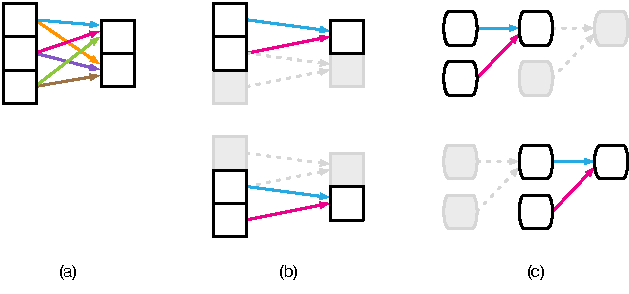
\includegraphics[width=\linewidth]{layers.pdf}
\end{figure}
\end{frame}

% ----------------------- Sets and Graphs -----------------------
\begin{frame}{Computations over Sets and Graphs}
\textbf{No standard DL component handles arbitrary relational structure.}
 
\vspace{0.3cm}
\begin{columns}[t]
\column{0.48\textwidth}
\footnotesize
\textbf{Sets} encode permutation invariance via symmetric aggregation (Deep Sets):
\begin{equation*}
    x'_i = f\!\left(x_i,\; \sum_j g(x_i, x_j)\right)
\end{equation*}
All pairs are considered; the prediction depends only on symmetric functions of the inputs.
 
\column{0.48\textwidth}
\footnotesize
\textbf{Graphs} extend this to \emph{sparse} pairwise structure:
\begin{equation*}
    x'_i = f\!\left(x_i,\; \sum_{j \in \delta(i)} g(x_i, x_j)\right)
\end{equation*}
where $\delta(i) \subseteq \{1, \ldots, n\}$ is the neighborhood of node $i$.
\end{columns}

\begin{figure}
    \centering
    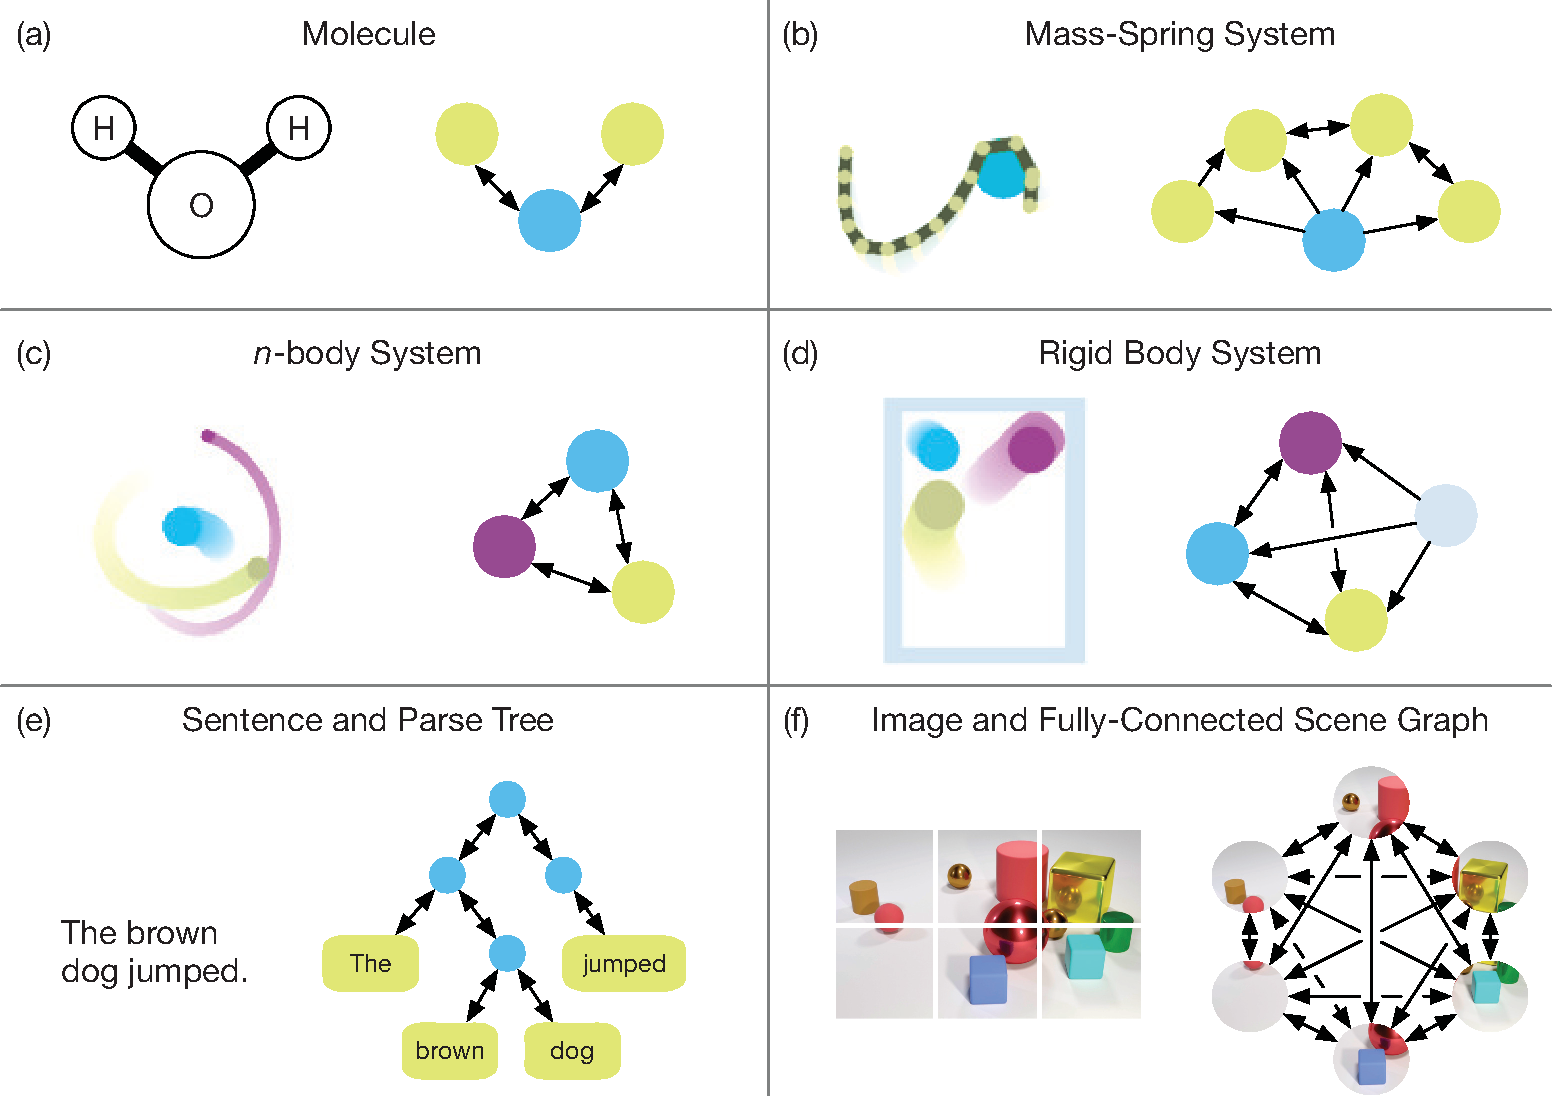
\includegraphics[width=0.80\linewidth]{graphs.pdf}
\end{figure}
\end{frame}
 

% ----------------------- GN Framework Definition -----------------------
\begin{frame}{Graph Network (GN) Framework: Definition}
A \textbf{graph} is a 3-tuple $G = (\mathbf{u}, V, E)$:
\begin{itemize}
    \item $\mathbf{u}$ --- global attribute (e.g.\ gravitational field).
    \item $V = \{\mathbf{v}_i\}_{i=1:N^v}$ --- node attributes (e.g.\ position, velocity, mass of each ball).
    \item $E = \{(\mathbf{e}_k, r_k, s_k)\}_{k=1:N^e}$ --- edge attributes with receiver index $r_k$ and sender index $s_k$ (e.g.\ spring constants).
\end{itemize}

\vspace{0.4cm}
The \textbf{GN block} is a \emph{graph-to-graph} module: takes $G$ as input,
performs computations over the structure, returns updated $G'$ as output.

\vspace{0.3cm}
\begin{block}{Three design principles}
\begin{enumerate}
    \item Flexible representations.
    \item Configurable within-block structure.
    \item Composable multi-block architectures.
\end{enumerate}
\end{block}
\end{frame}

% ----------------------- GN Block Structure -----------------------
\begin{frame}{GN Block: Update and Aggregation Functions}
A GN block contains three \textbf{update} ($\phi$) and three \textbf{aggregation} ($\rho$) functions:
\begin{align*}
    \mathbf{e}'_k &= \phi^e(\mathbf{e}_k,\, \mathbf{v}_{r_k},\, \mathbf{v}_{s_k},\, \mathbf{u}) \\[2pt]
    \mathbf{v}'_i &= \phi^v(\bar{\mathbf{e}}'_i,\, \mathbf{v}_i,\, \mathbf{u}) \\[2pt]
    \mathbf{u}'  &= \phi^u(\bar{\mathbf{e}}',\, \bar{\mathbf{v}}',\, \mathbf{u})
\end{align*}
\begin{equation*}
    \bar{\mathbf{e}}'_i = \rho^{e \to v}(E'_i), \qquad
    \bar{\mathbf{e}}' = \rho^{e \to u}(E'), \qquad
    \bar{\mathbf{v}}' = \rho^{v \to u}(V')
\end{equation*}

\textbf{Computation order:} edge updates $\to$ node updates $\to$ global update.

\begin{columns}
\column{0.55\textwidth}
The $\rho$ functions must be \emph{permutation invariant} and accept variable
numbers of inputs (e.g.\ elementwise sum, mean, max).
\column{0.42\textwidth}
\begin{figure}
    \centering
    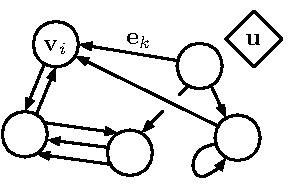
\includegraphics[width=\linewidth]{graph.pdf}
\end{figure}
\end{columns}
\end{frame}

% ----------------------- Neural Network Implementation -----------------------
\begin{frame}{Full GN Block: Neural Network Implementation}
\textbf{$\phi$ functions implemented as neural networks} ($\mathrm{NN}^e$, $\mathrm{NN}^v$, $\mathrm{NN}^u$):
\begin{align*}
    \phi^e(\mathbf{e}_k, \mathbf{v}_{r_k}, \mathbf{v}_{s_k}, \mathbf{u})
        &:= \mathrm{NN}^e\!\left([\mathbf{e}_k,\, \mathbf{v}_{r_k},\, \mathbf{v}_{s_k},\, \mathbf{u}]\right) \\[2pt]
    \phi^v(\bar{\mathbf{e}}'_i, \mathbf{v}_i, \mathbf{u})
        &:= \mathrm{NN}^v\!\left([\bar{\mathbf{e}}'_i,\, \mathbf{v}_i,\, \mathbf{u}]\right) \\[2pt]
    \phi^u(\bar{\mathbf{e}}', \bar{\mathbf{v}}', \mathbf{u})
        &:= \mathrm{NN}^u\!\left([\bar{\mathbf{e}}',\, \bar{\mathbf{v}}',\, \mathbf{u}]\right)
\end{align*}

\textbf{$\rho$ functions implemented as elementwise summation:}
\begin{equation*}
    \rho^{e \to v}(E'_i) := \!\!\sum_{\{k:\, r_k = i\}}\!\! \mathbf{e}'_k, \quad
    \rho^{v \to u}(V') := \sum_i \mathbf{v}'_i, \quad
    \rho^{e \to u}(E') := \sum_k \mathbf{e}'_k
\end{equation*}

\vspace{0.2cm}
$[\cdot,\, \cdot]$ denotes concatenation. MLPs are used for vector attributes;
CNNs for tensor attributes (e.g.\ image feature maps). The $\phi$ functions
can also be \emph{RNNs} with an additional hidden state.
\end{frame}

% ----------------------- GN Variants -----------------------
\begin{frame}{GN Variants: Configurable Within-Block Structure}
Many published architectures are special cases of the GN framework:

\begin{itemize}
    \item \textbf{MPNN}: $\phi^e$ omits $\mathbf{u}$; readout $R$ plays role of
    $\phi^u$ without taking $\mathbf{u}$ or $E'$ as input.\footnote{
        Gilmer, J., Schoenholz, S. S., Riley, P. F., Vinyals, O., and Dahl, G. E. (2017). Neural message passing for quantum chemistry.
    }
    \item \textbf{NLNN / Self-Attention}:
    $\phi^e$ factored into scalar attention weight $\alpha^e(\mathbf{v}_{r_k}, \mathbf{v}_{s_k})$
    and value $\beta^e(\mathbf{v}_{s_k})$; only nodes are output.\footnote{
        Wang, X., Girshick, R., Gupta, A., and He, K. Non-local neural networks.
    }\footnote{
        Vaswani, A., Shazeer, N., Parmar, N., Uszkoreit, J., Jones, L., Gomez, A. N., Kaiser, L., and Polosukhin, I. Attention is all you need. 
    }
    \item \textbf{Relation Networks} (Santoro et al., 2017): node update bypassed;
    global predicted directly from pooled edge representations.\footnote{
        Santoro, A., Raposo, D., Barrett, D. G., Malinowski, M., Pascanu, R., Battaglia, P., and Lillicrap, T. A simple neural network module for relational reasoning.
    }
    \item \textbf{Deep Sets}: edge update bypassed;
    global predicted directly from pooled node representations.\footnote{
        Zaheer, M., Kottur, S., Ravanbakhsh, S., Poczos, B., Salakhutdinov, R. R., and Smola, A. J. Deep sets. 
    }
\end{itemize}
\end{frame}

% ----------------------- Composable Architectures -----------------------
\begin{frame}{Composable Multi-Block Architectures}
\textbf{GN blocks compose naturally} via their graph-to-graph interface:
\begin{equation*}
    G' = \mathrm{GN}_2(\mathrm{GN}_1(G))
\end{equation*}

\textbf{Shared} ($\mathrm{GN}_1 = \cdots = \mathrm{GN}_M$): analogous to unrolled
RNN / message-passing; information propagates $m$ hops after $m$ steps.

\textbf{Unshared} ($\mathrm{GN}_1 \neq \cdots \neq \mathrm{GN}_M$): analogous to
layers of a CNN.

\vspace{0.3cm}
\begin{block}{Encode-process-decode (most common design)}
\begin{enumerate}
    \item $\mathrm{GN}_{\mathrm{enc}}$ maps input graph $G_{\mathrm{inp}}$ to latent graph $G_0$.
    \item Shared $\mathrm{GN}_{\mathrm{core}}$ is applied $M$ times.
    \item $\mathrm{GN}_{\mathrm{dec}}$ maps result to output graph $G_{\mathrm{out}}$.
\end{enumerate}
\end{block}
\end{frame}

% ----------------------- Relational Inductive Biases in GNs -----------------------
\begin{frame}{Relational Inductive Biases in Graph Networks}
GNs impose \textbf{three strong relational inductive biases:}

\vspace{0.3cm}
\textbf{1.\ Arbitrary relational structure.}
\begin{itemize}
    \item Edges define which entities interact; absence of an edge means no direct influence.
    \item The \emph{input graph} determines interactions, not a fixed architecture.
\end{itemize}

\vspace{0.3cm}
\textbf{2.\ Permutation invariance.}
\begin{itemize}
    \item Entities and relations are represented as sets.
    \item GN output is invariant to the ordering of nodes and edges.
\end{itemize}

\vspace{0.3cm}
\textbf{3.\ Per-edge and per-node function reuse.}
\begin{itemize}
    \item The same $\phi^e$ and $\phi^v$ are applied across \emph{all} edges and nodes.
    \item A single GN operates on graphs of different sizes (node/edge counts) and shapes (connectivity).
    \item Directly underpins combinatorial generalization.
\end{itemize}
\end{frame}

% ----------------------- Combinatorial Generalization Results -----------------------
\begin{frame}{Combinatorial Generalization in Graph Networks}
\textbf{Entity- and relation-centric structure directly supports out-of-distribution generalization:}

\begin{itemize}
    \item \textbf{Physical simulation} (Battaglia et al., 2016): trained for one-step prediction,
    GNs simulate thousands of future steps; zero-shot transfer to $2\times$/$0.5\times$ as many entities.
    \item \textbf{Multi-joint control} (Sanchez-Gonzalez et al., 2018): forward models
    generalize to agents with unseen numbers of joints.
    \item \textbf{Combinatorial optimization} (Bello et al., 2016; Dai et al., 2017):
    generalize well to problem sizes far outside the training distribution.
    \item \textbf{Boolean SAT} (Selsam et al., 2018): retains performance across different
    problem sizes \emph{and} input graph distributions.
\end{itemize}

\end{frame}

% ----------------------- Limitations and Open Questions -----------------------
\begin{frame}{Limitations and Open Questions}
\textbf{Known limitations:}
\begin{itemize}
    \item Learned message-passing cannot discriminate all non-isomorphic graphs
    (Shervashidze et al., 2011).
    \item Recursion, control flow, and conditional iteration are not natively
    representable as graphs.
\end{itemize}

\vspace{0.3cm}
\textbf{Open questions:}
\begin{itemize}
    \item \textbf{Graph construction:} converting raw sensory data (images, text)
    into a sparse, meaningful graph structure remains unsolved.
    \item \textbf{Adaptive structure:} how to add or remove nodes and edges
    dynamically during computation (e.g.\ object fracturing).
\end{itemize}
\end{frame}

% ----------------------- Conclusion -----------------------
\begin{frame}{Conclusion}
\begin{block}{What graph networks deliver}
A principled framework for relational reasoning that unifies and extends prior
work on graph neural networks while combining the strengths of structured
approaches and end-to-end deep learning.
\end{block}

\vspace{0.1cm}
\textbf{The argument:}
\begin{itemize}
    \item Combinatorial generalization is a top priority for AI.
    \item Standard DL components have limited relational inductive biases.
    \item GNs impose strong relational structure while remaining fully learnable.
\end{itemize}

\vspace{0.1cm}
\textbf{Three design principles:}
\begin{itemize}
    \item Flexible attribute representations (vectors, tensors, graphs).
    \item Configurable within-block structure (unifies MPNN, NLNN, Relation Nets, Deep Sets).
    \item Composable multi-block architectures (encode-process-decode, recurrent GN).
\end{itemize}
\end{frame}

\end{document}